\documentclass[conference]{IEEEtran}
\usepackage[T1]{fontenc}
\usepackage[utf8]{inputenc}
\usepackage{amsmath,amssymb}
\usepackage{booktabs}
\usepackage{cite}
\usepackage{graphicx}
\usepackage{tabularx}
\usepackage{url}

\graphicspath{{figures/}}
\newcommand{\DatasetAnnotationCount}{1014}
\newcommand{\DatasetPatientCount}{53}
\newcommand{\DatasetTrialCount}{103}
\newcommand{\TrainPatientCount}{37}
\newcommand{\TrainAnnotationCount}{602}
\newcommand{\ValPatientCount}{8}
\newcommand{\ValAnnotationCount}{206}
\newcommand{\TestPatientCount}{8}
\newcommand{\TestAnnotationCount}{206}
\newcommand{\ValidationHeadlineMacroFone}{0.5500}
\newcommand{\TestHeadlineAccuracy}{\textit{pending final evaluation}}
\newcommand{\TestHeadlineMacroFone}{\textit{pending final evaluation}}
\newcommand{\TestHeadlineAccuracyCI}{--}
\newcommand{\TestHeadlineMacroFoneCI}{--}


\title{CriterionLens: Evidence-Grounded Criterion-Level Clinical Trial Matching with Small Language Models}
\author{\IEEEauthorblockN{Syed Ashher Majid}
\IEEEauthorblockA{FAST-NUCES Islamabad\\
\texttt{i230007@isb.nu.edu.pk}}}

\begin{document}
\maketitle

\begin{abstract}
Clinical-trial eligibility matching requires a separate, evidence-grounded judgment for each criterion, including an explicit way to abstain when a note is incomplete. CriterionLens fine-tunes compact instruction models to return a structured label and numbered supporting sentences, and pairs the screening pipeline with explicit KV-cache, tiled-attention, and greedy speculative-decoding implementations. On the fixed held-out split, the fine-tuned 1.5B model obtains accuracy \TestHeadlineAccuracy{} and fixed-label macro-F1 \TestHeadlineMacroFone{} (bootstrap 95\% intervals \TestHeadlineAccuracyCI{} and \TestHeadlineMacroFoneCI{}). These results characterize a small research prototype on a limited annotated dataset; they do not establish clinical utility. The official application is browser-accessible and locally hosted, as permitted by the assignment.
\end{abstract}

\begin{IEEEkeywords}
clinical trial matching, evidence extraction, language models, parameter-efficient fine-tuning, inference
\end{IEEEkeywords}

\section{Introduction}
Clinical-trial screening compares a patient's clinical history with many protocol eligibility criteria. A trial-level decision can hide which individual requirement was supported, contradicted, or left unknown. Prior work has therefore framed matching as criterion-level classification and explanation \cite{jin2024trialgpt,koopman2016collection}. CriterionLens follows that framing but targets a small, locally runnable decoder and returns sentence identifiers rather than an unconstrained rationale.

The system has four contributions. First, it fine-tunes Qwen2.5 instruction models with completion-only LoRA updates and evaluates them on a patient-disjoint split. Second, it extracts numbered evidence, validates output schemas, and treats missing information and unsupported decisive labels conservatively. Third, it implements and measures explicit KV-cached generation, tiled online-softmax attention, and greedy speculative decoding. Fourth, it packages these components in a local Gradio application that is explicitly a research aid, not a medical device.

\section{Problem formulation}
Given a numbered patient note $x$ and one inclusion or exclusion criterion $c$, the model predicts an allowed criterion-type-specific label $y$ and a set of supporting sentence IDs $E$. The label includes a not-enough-information option; absent evidence is not interpreted as proof of eligibility or ineligibility. A later aggregation rule produces only a preliminary trial-level summary and routes unresolved cases to manual review.

\section{Related Work}
\subsection{Patient-to-trial matching}
TrialGPT structures matching around criterion-level judgments and explanations \cite{jin2024trialgpt}. The SIGIR clinical-trial collection provides a reproducible benchmark for patient-to-trial matching \cite{koopman2016collection}. These resources motivate explicit criterion-level output, but benchmark performance alone cannot establish safe enrollment decisions. CriterionLens therefore exposes evidence and abstention and makes no clinical-use claim.

\subsection{Transformers and parameter-efficient adaptation}
Self-attention provides parallel sequence modeling but its full attention matrix scales quadratically with sequence length \cite{vaswani2017attention}. Qwen2.5 is an open-weight instruction-model family \cite{yang2025qwen25}; its rotary positions and grouped-query attention inform the decoding implementation \cite{su2021roformer,ainslie2023gqa}. LoRA learns low-rank updates while freezing base weights \cite{hu2022lora}. QLoRA is a memory-saving alternative, but was not required for the selected training runs \cite{dettmers2023qlora}.

\subsection{Efficient inference}
The KV cache avoids recomputing prior keys and values during autoregressive generation; grouped-query attention reduces its size. Online softmax and FlashAttention motivate tiled attention that avoids materializing the full score matrix \cite{milakov2018online,dao2022flashattention}. PagedAttention addresses serving-time cache management at a different systems level \cite{kwon2023pagedattention}. Speculative decoding uses a draft model and target verification, with realized speed depending on acceptance and hardware \cite{leviathan2023speculative}. The implementations here are measured independently; theoretical efficiency is not treated as an empirical speedup.

\section{Data and Model Selection}
\subsection{Dataset and audit}
The experiments use the public TrialGPT criterion-annotation dataset \cite{jin2024trialgpt}. The audit retained \DatasetAnnotationCount{} annotations from \DatasetPatientCount{} patients and \DatasetTrialCount{} trials after dropping empty criterion text. GPT-4-generated explanations and labels were excluded at load time; training targets use only expert eligibility labels and expert evidence sentence IDs. The fixed split is patient-disjoint, with seed 42 and counts shown in Table~\ref{tab:split}.

\begin{table}[t]
\centering
\caption{Patient-disjoint dataset partition sizes.}
\label{tab:split}
\begin{tabular}{lrrrr}
\toprule
Split & Patients & Annotations & Inclusion & Exclusion \\
\midrule
TRAIN & 37 & 602 & 215 & 387 \\
VAL & 8 & 206 & 66 & 140 \\
TEST & 8 & 206 & 75 & 131 \\
\bottomrule
\end{tabular}
\end{table}

\begin{table}[t]
\centering
\caption{LoRA training configuration read from the versioned YAML files.}
\label{tab:hyperparameters}
\begin{tabular}{lrrrrrr}
\toprule
Model & Max tokens & Epochs & Batch x accum. & Rank/alpha & Learning rate & Seed \\
\midrule
1.5B & 640 & 3 & 4 x 4 & 16/32 & 2.0e-04 & 42 \\
0.5B & 640 & 3 & 4 x 4 & 16/32 & 2.0e-04 & 42 \\
\bottomrule
\end{tabular}
\end{table}


The split is frozen by a manifest containing the dataset revision and patient assignments. All prompt, training, and model comparisons use the same split; the held-out test partition is accessed only by the tagged final evaluation.

\subsection{Models and supervised fine-tuning}
Qwen2.5-1.5B-Instruct is the primary target and Qwen2.5-0.5B-Instruct is the size comparison and same-tokenizer draft \cite{yang2025qwen25}. LoRA updates query, key, value, output, and MLP projections while the base weights remain frozen \cite{hu2022lora}. The training target is a compact JSON object with evidence IDs followed by a criterion-type-specific label. The patient note is placed before the criterion; explanations are generated from cited text by a deterministic template, not learned from GPT-4 columns.

Training histories record optimization loss and validation loss by epoch. They do not contain generation-based validation F1 for every checkpoint. Therefore, the report compares the completed final adapters on the already-run fixed validation evaluations and does not claim an epoch was selected by generation F1 (D-006).
The versioned training settings are summarized in Table~\ref{tab:hyperparameters}.

\section{Criterion-Level Inference and Decoding}
\subsection{Structured prediction and evidence}
The instruction prompt requests one JSON object. The parser validates the label against the criterion type, removes and records out-of-range sentence IDs, and invokes constrained label scoring if generation cannot be parsed. A decisive prediction without evidence is marked unsupported. A grounded template explains the output using only cited sentences; the aggregation rule treats unsupported or unknown criteria as requiring review rather than as a pass.

\subsection{KV-cached autoregressive decoding}
The reference decoder recomputes the full prefix. The cached decoder prefills a Hugging Face dynamic cache once, then forwards one token per step with the absolute position and an expanded attention mask. With $L$ layers, $H_{kv}$ key/value heads, head dimension $d_h$, sequence length $S$, batch $B$, and $b$ bytes per element, the cache allocation is
\begin{equation}
M_{KV}=2L B H_{kv} S d_h b.
\end{equation}
The factor two accounts for keys and values. Tests check token equality on tiny models, cache growth, byte counts, and a negative position-reset case. Timing and allocation are measured separately from correctness.
Figure~\ref{fig:kv-flow} shows that the cache is extended with each token and reused by the next decode step.

\begin{figure*}[t]
\centering
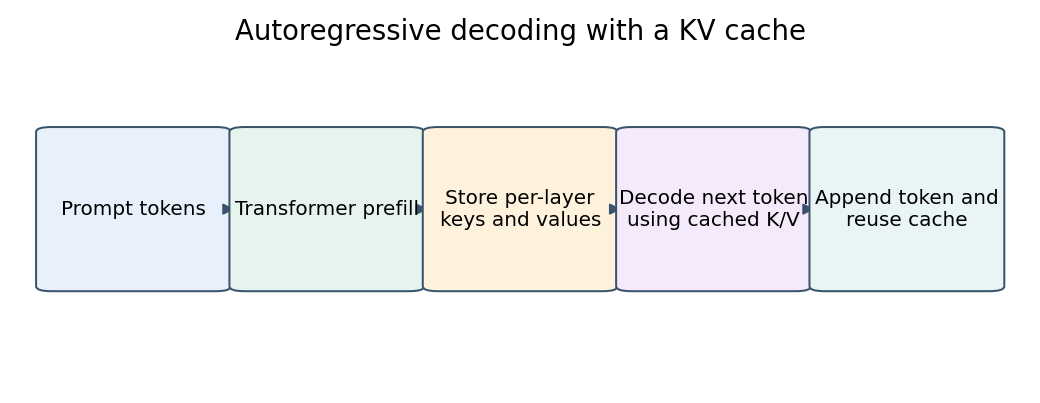
\includegraphics[width=\textwidth]{kv_cache_flow.png}
\caption{KV-cached autoregressive decoding: the prefix is prefetched once and each generated token extends the per-layer key/value cache.}
\label{fig:kv-flow}
\end{figure*}

\subsection{Tiled online-softmax attention}
The tiled implementation traverses query and key blocks and maintains a running row maximum $m$, normalizer $\ell$, and weighted-value accumulator $a$. When a new key tile changes the maximum from $m$ to $m'$, prior accumulators are rescaled by $\alpha=\exp(m-m')$, and the tile contributes its own normalized weights. The final output is $a/\ell$. This avoids storing the full score matrix while keeping accumulation in higher precision. Numerical error is compared with a double-precision reference; fused SDPA methods are performance baselines, not the implementation under test.
Figure~\ref{fig:tiled-flow} illustrates the online rescaling that permits blockwise accumulation without materializing the full score matrix.

\begin{figure*}[t]
\centering
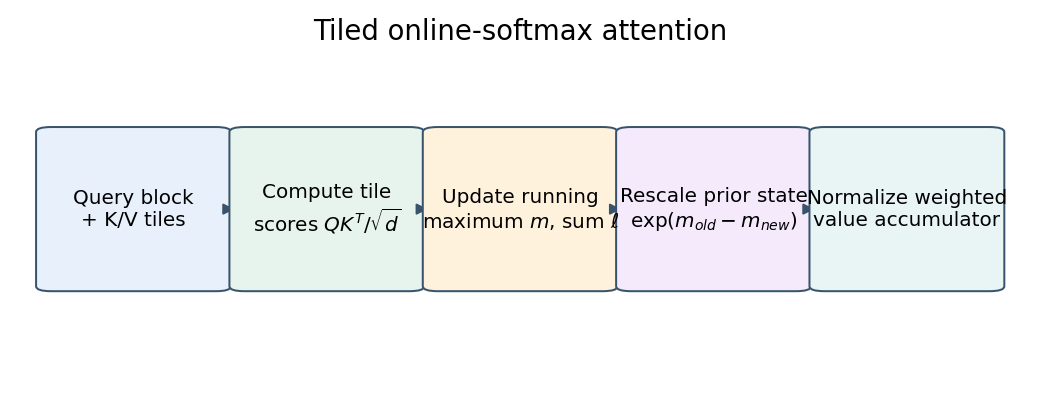
\includegraphics[width=\textwidth]{tiled_attention_flow.png}
\caption{Tiled attention maintains an online softmax state and rescales it when the running maximum changes.}
\label{fig:tiled-flow}
\end{figure*}

\subsection{Greedy speculative decoding}
The smaller model proposes up to $k$ tokens, then the target verifies the proposed block. Matching target argmax tokens are accepted; at the first mismatch the target token is emitted and the draft cache is cropped to the accepted prefix. The method is greedy and is checked for exact output equality against target KV-cache decoding. Acceptance rate and timing are reported independently because matching tokens need not yield a speedup on every hardware configuration.
Figure~\ref{fig:speculative-flow} depicts the accepted-prefix and target-correction steps for greedy decoding.

\begin{figure*}[t]
\centering
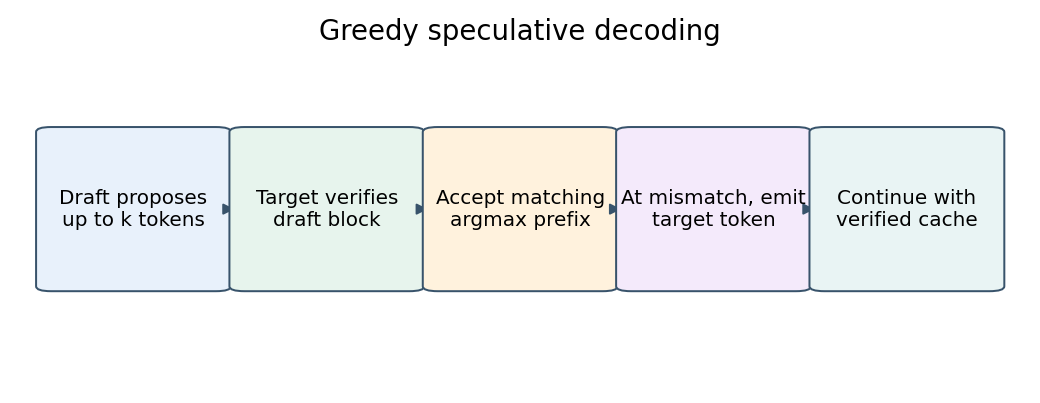
\includegraphics[width=\textwidth]{speculative_decoding_flow.png}
\caption{Greedy speculative decoding proposes a block, accepts the matching prefix, and uses the target token at the first mismatch.}
\label{fig:speculative-flow}
\end{figure*}

\section{Experimental Setup and Metrics}
The training and benchmark kernels requested two NVIDIA Tesla T4 GPUs on Kaggle. Each benchmark process measures one model at a time; the two-GPU allocation is not described as data-parallel inference. The laptop environment was used for unit tests and application work. The exact software versions, model identifiers, dtype, device, timing repetitions, and input source are retained in the result JSON files.

Classification reports accuracy, observed-label macro-F1, fixed-label macro-F1, per-class scores, and confusion matrices. For the final test split, criterion-level accuracy and macro-F1 receive percentile bootstrap 95\% intervals from 1,000 resamples with seed 42. Evidence extraction reports micro scores and primary macro scores over records with non-empty expert evidence; empty-gold abstention accuracy and invalid sentence IDs are reported separately.

KV-cache benchmarks use deterministic synthetic token IDs, two warm-ups, and five timed repeats per grid point; they compare full-prefix recomputation with cached decoding. Tiled attention uses deterministic random query/key/value tensors and records accuracy and performance grids, including unavailable fused backends and out-of-memory cases. Speculative-decoding benchmarks use deterministic synthetic prompts, two warm-ups, five repeats, two output lengths, and multiple values of $k$. These synthetic workloads measure inference mechanics, not clinical matching quality.

The final evaluation uses greedy no-cache decoding with 64 generated tokens on the four predeclared base/adapter combinations. The final kernel requires a verified freeze manifest for tag \texttt{v1.0-frozen}; each pair is guarded against repeat access in the access log.

\section{Results}
\subsection{Classification and evidence}
Table~\ref{tab:main-results} is generated directly from the four recovered validation outputs and the one-time final test outputs. The headline test values and their bootstrap intervals are reported in the abstract. Figure~\ref{fig:classification} compares accuracy and fixed-label macro-F1 with criterion-level bootstrap intervals; Fig.~\ref{fig:per-class} shows per-class behavior. Confusion matrices are saved for every evaluated model; the headline model's test confusion matrix is included below.

Fine-tuning is the dominant factor. On the held-out test patients, LoRA fine-tuning raises accuracy from 0.204 to 0.762 for the 1.5B model and from 0.325 to 0.694 for the 0.5B model, and fixed-label macro-F1 from 0.158 to 0.476 and from 0.093 to 0.410. Both fine-tuned models produced parseable JSON for all 206 test criteria, while the base 0.5B model failed to parse on 1.0\% of them. The base models fail in characteristic ways. Base 1.5B labels 109 of 206 test criteria \emph{not applicable} (gold: 15) and predicts \emph{excluded} 32 times when no test criterion carries that gold label. Base 0.5B almost always abstains. Model scale matters less than supervision: the fine-tuned 0.5B outperforms the base 1.5B by a wide margin, and the 1.5B adds about 7 accuracy points over the fine-tuned 0.5B. Validation and test results agree closely (fine-tuned 1.5B accuracy 0.748 vs.\ 0.762), so the selected checkpoint does not appear over-fitted to the validation patients. For evidence, the fine-tuned 1.5B reaches micro-F1 0.542 and primary macro-F1 0.584 (Table~\ref{tab:evidence-results}), and no model cited a sentence ID outside the note.

\begin{table}[t]
\centering
\caption{Criterion-level bootstrap 95\% confidence intervals (1,000 resamples; seed 42).}
\label{tab:main-results}
\begin{tabular}{lrrrrr}
\toprule
Split & Model & Accuracy & Macro-F1 & Accuracy CI & Macro-F1 CI \\
\midrule
VAL & Base 0.5B & 0.257 & 0.084 & [0.204, 0.320] & [0.061, 0.111] \\
VAL & Base 1.5B & 0.267 & 0.204 & [0.209, 0.330] & [0.165, 0.243] \\
VAL & Fine-tuned 0.5B & 0.714 & 0.432 & [0.650, 0.777] & [0.365, 0.487] \\
VAL & Fine-tuned 1.5B & 0.748 & 0.550 & [0.689, 0.806] & [0.394, 0.646] \\
\bottomrule
\end{tabular}
\end{table}

\begin{table}[t]
\centering
\caption{Evidence-set scores; primary macro-F1 averages records with non-empty expert evidence.}
\label{tab:evidence-results}
\begin{adjustbox}{max width=\columnwidth}
\begin{tabular}{lrrrrr}
\toprule
Split & Model & Micro-F1 & Primary macro-F1 & Empty gold & Abstention acc. \\
\midrule
TEST & Base 0.5B & 0.020 & 0.007 & 145 & 1.000 \\
TEST & Base 1.5B & 0.242 & 0.498 & 145 & 0.000 \\
TEST & Fine-tuned 0.5B & 0.473 & 0.526 & 145 & 0.890 \\
TEST & Fine-tuned 1.5B & 0.542 & 0.584 & 145 & 0.897 \\
VAL & Base 0.5B & 0.030 & 0.009 & 116 & 0.991 \\
VAL & Base 1.5B & 0.216 & 0.409 & 116 & 0.000 \\
VAL & Fine-tuned 0.5B & 0.420 & 0.470 & 116 & 0.888 \\
VAL & Fine-tuned 1.5B & 0.546 & 0.616 & 116 & 0.853 \\
\bottomrule
\end{tabular}
\end{adjustbox}
\end{table}

\begin{table}[t]
\centering
\caption{Per-class precision, recall, and F1 for val ft 1p5b.}
\label{tab:per-class}
\begin{tabular}{lrrrr}
\toprule
Label & Precision & Recall & F1 & Support \\
\midrule
included & 0.800 & 0.686 & 0.738 & 35 \\
not included & 0.000 & 0.000 & 0.000 & 3 \\
not enough information & 0.622 & 0.528 & 0.571 & 53 \\
not applicable & 0.500 & 0.417 & 0.455 & 12 \\
excluded & 1.000 & 0.500 & 0.667 & 2 \\
not excluded & 0.800 & 0.950 & 0.869 & 101 \\
\bottomrule
\end{tabular}
\end{table}


\begin{figure}[t]
\centering
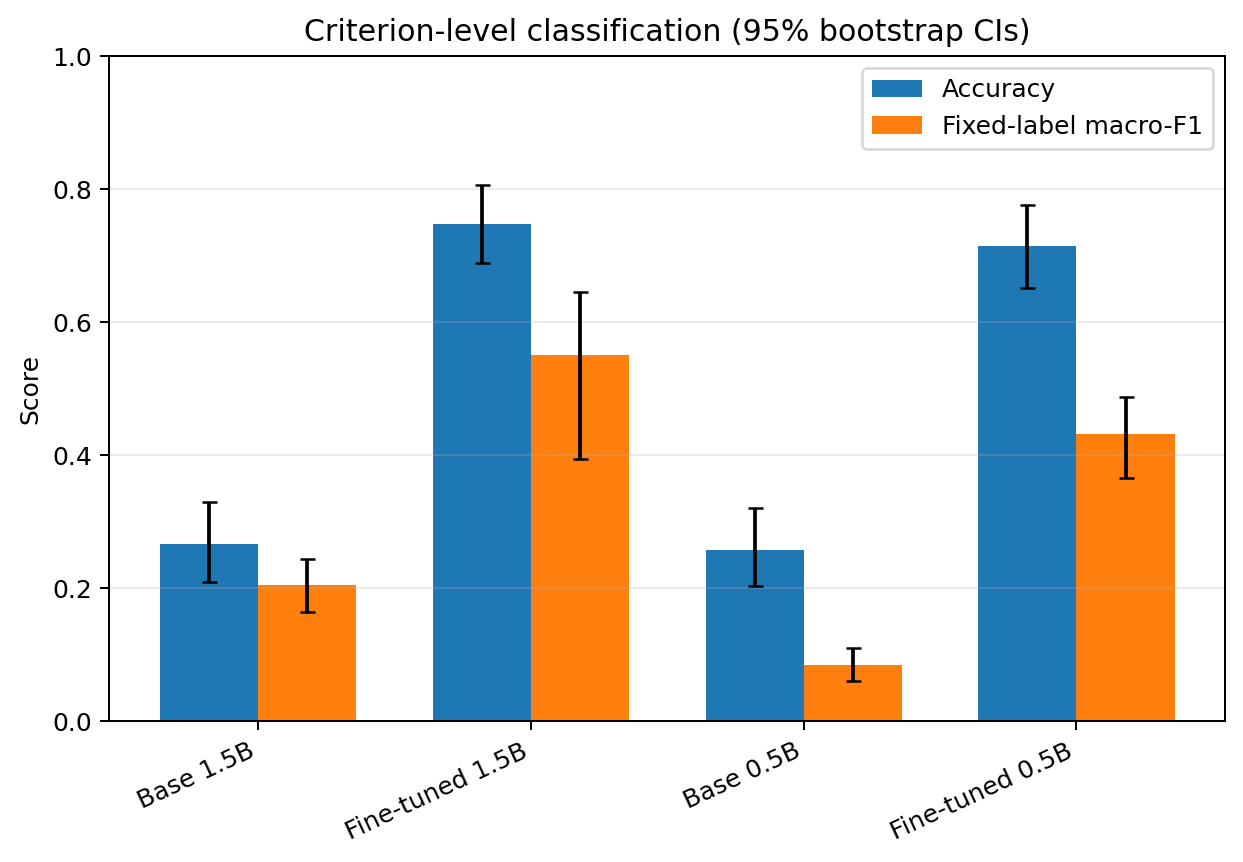
\includegraphics[width=\columnwidth]{classification_metrics.png}
\caption{Accuracy and fixed-label macro-F1 across validation and final test evaluations.}
\label{fig:classification}
\end{figure}

\begin{figure}[t]
\centering
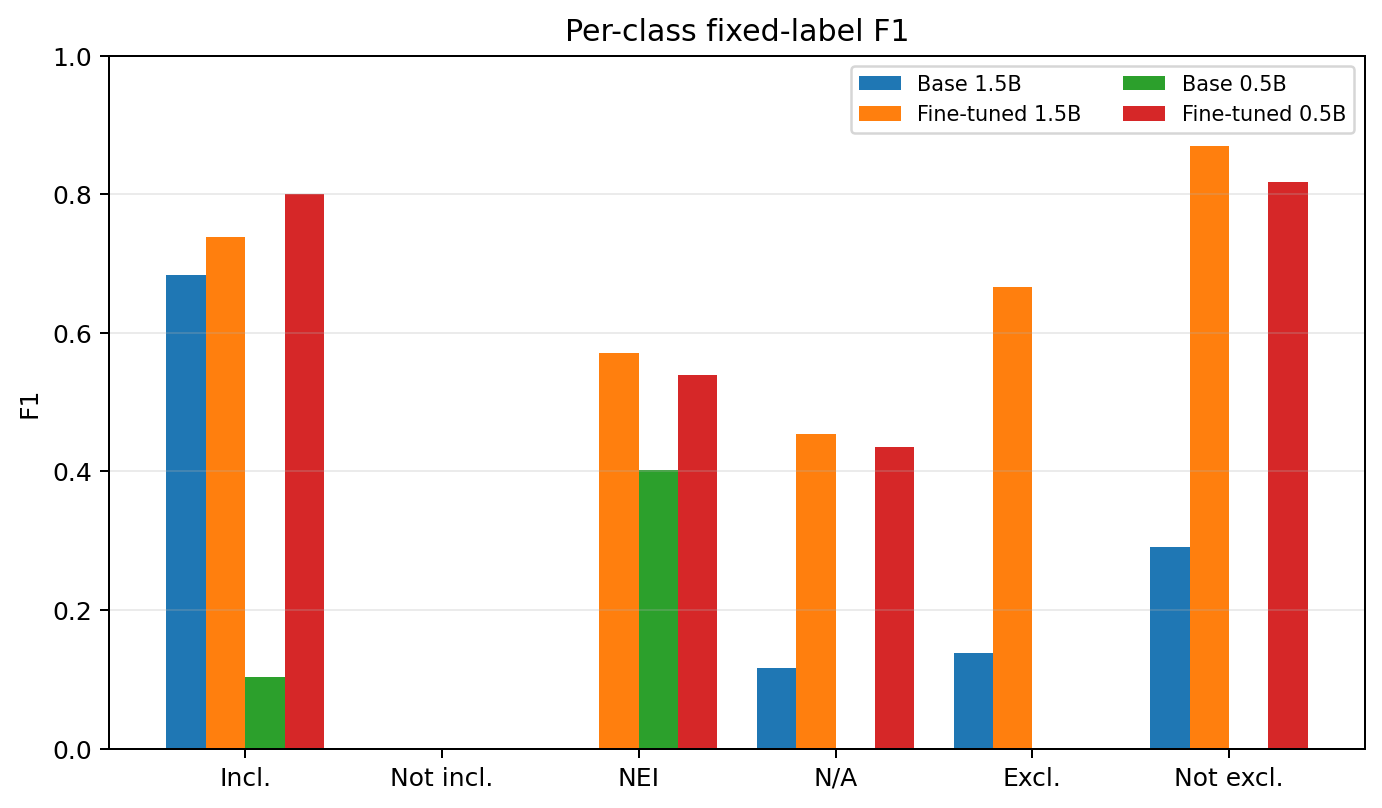
\includegraphics[width=\columnwidth]{per_class_f1.png}
\caption{Per-class F1 across the evaluated base and fine-tuned variants.}
\label{fig:per-class}
\end{figure}

\begin{figure}[t]
\centering
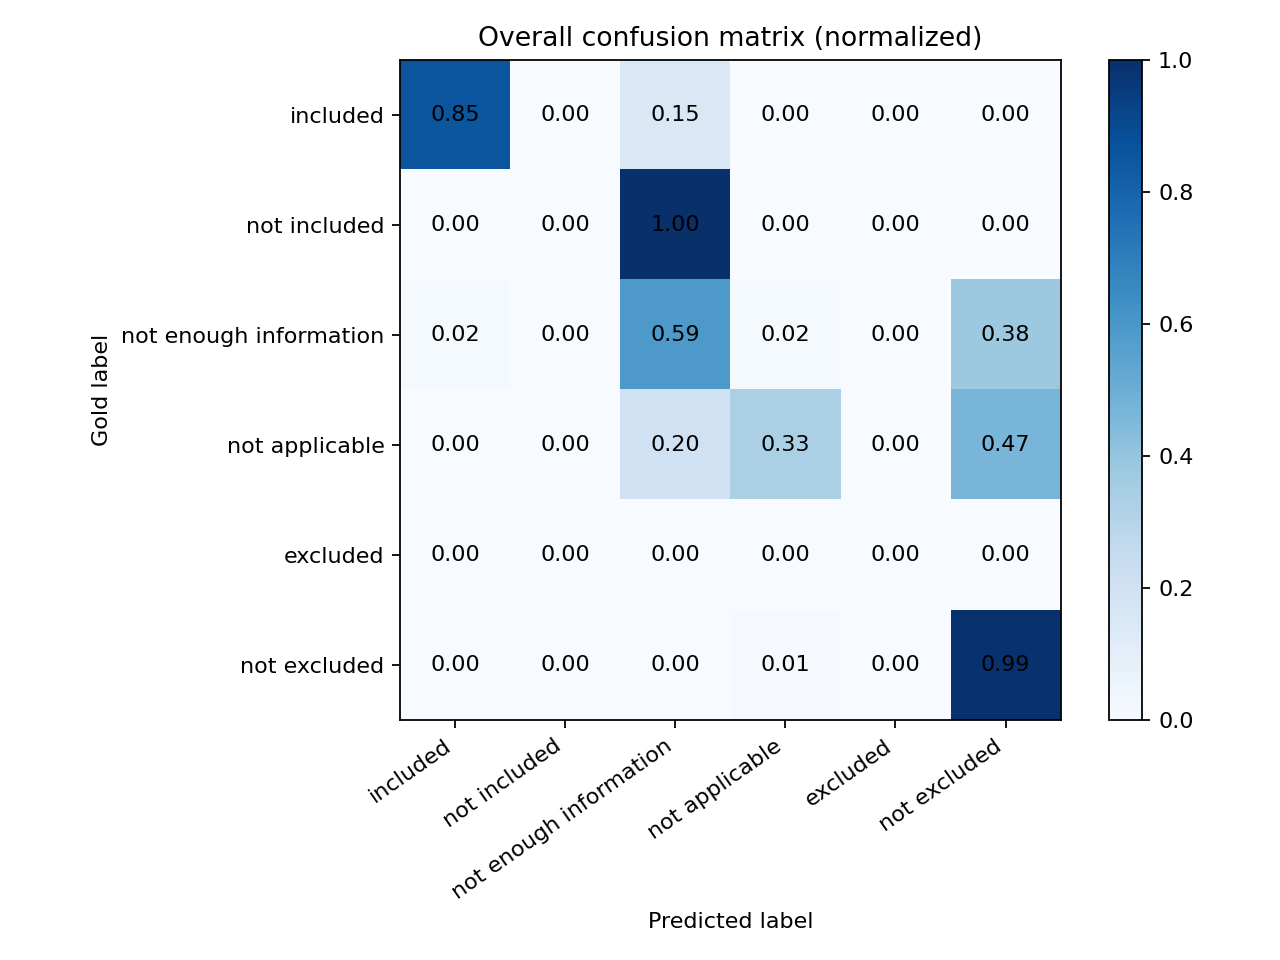
\includegraphics[width=\columnwidth]{test_ft_1p5b_confusion_overall_normalized.png}
\caption{Row-normalized six-label confusion matrix for the fine-tuned 1.5B headline model on the fixed test set.}
\label{fig:headline-confusion}
\end{figure}

The validation comparison selected the final fine-tuned 1.5B adapter as the headline model (fixed-label macro-F1 \ValidationHeadlineMacroFone{}); this is a comparison among final adapters, not per-epoch checkpoint selection. Evidence metrics and empty-gold conventions are shown in Table~\ref{tab:evidence-results}.

\subsection{Training dynamics}
Figure~\ref{fig:training} plots the logged optimization loss and validation loss. The available histories do not contain generation-based F1 for each epoch, so no epoch-level F1 curve is inferred.
\begin{figure}[t]
\centering
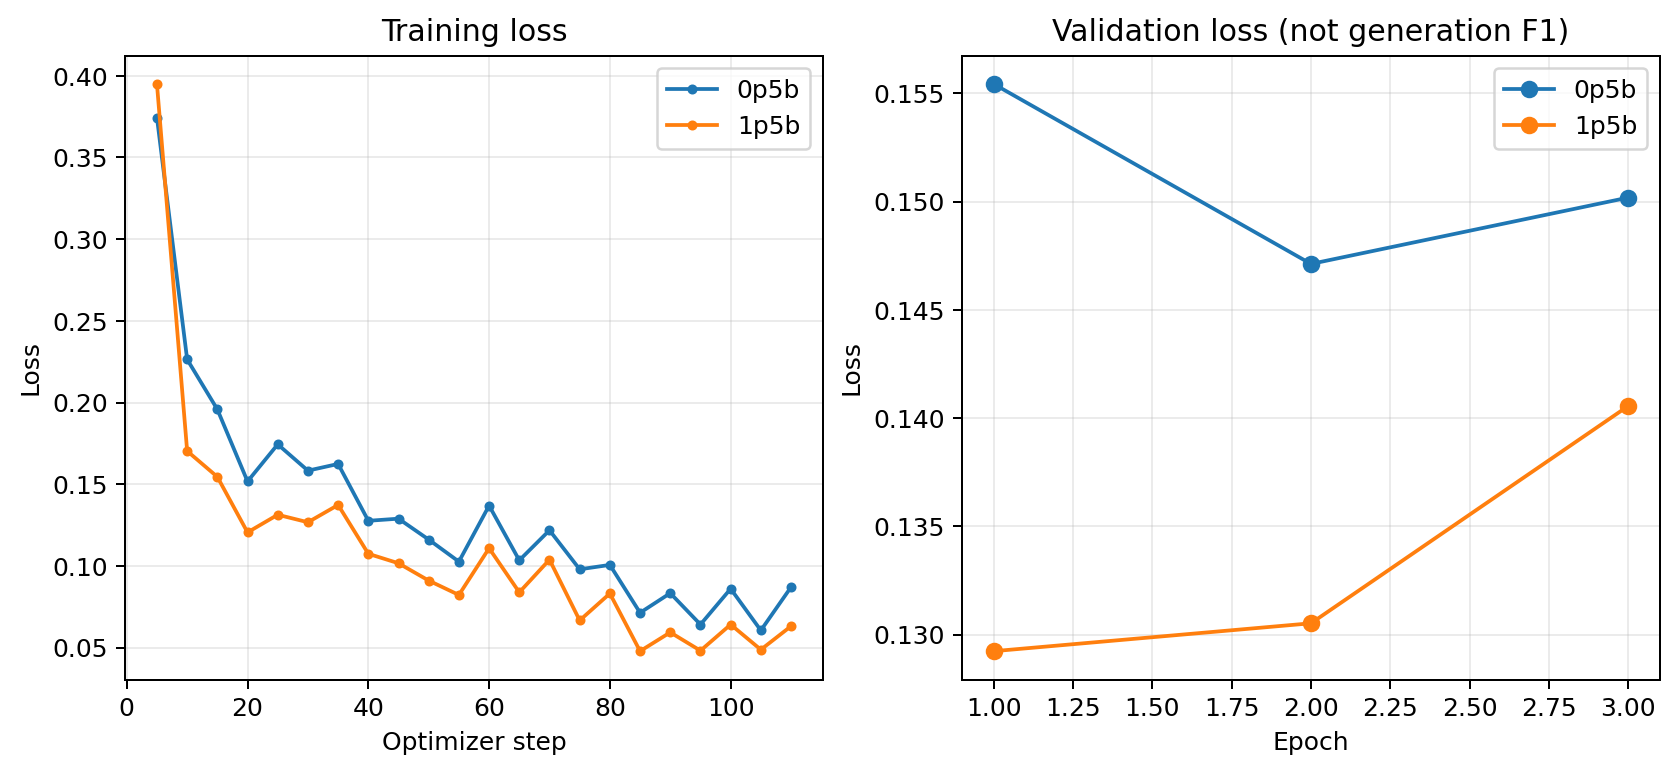
\includegraphics[width=\columnwidth]{training_curves.png}
\caption{Training and recorded validation loss; validation generation F1 was not logged per epoch.}
\label{fig:training}
\end{figure}

\subsection{Inference benchmarks}
The KV-cache results report latency, decode throughput, peak allocation, and measured cache growth; Table~\ref{tab:kv-results} and Figs.~\ref{fig:kv-latency}--\ref{fig:kv-growth} are generated from the benchmark JSON. The tiled-attention error table (Table~\ref{tab:attention-accuracy}) and performance plots distinguish successful, unavailable, and OOM rows. Speculative acceptance, speedup, and latency are plotted against $k$ separately for each draft and output length (Table~\ref{tab:speculative}). No speedup is asserted without the corresponding measured result.

All benchmarks ran on one Kaggle Tesla T4 (PyTorch 2.11, Transformers 4.57.6) with one warm-up and three timed repeats for KV and attention, and two repeats for speculative decoding. \emph{KV cache.} For the fine-tuned 1.5B model in float16, generating 128 tokens after a 1024-token prompt took 46.4\,s with full-prefix recomputation and 4.72\,s with our KV cache (2.76 vs.\ 29.1 output tokens/s; 9.8$\times$). The gain grows with context: 1.5$\times$, 4.9$\times$ and 9.8$\times$ at 128, 512 and 1024 input tokens (1.1$\times$, 2.5$\times$ and 6.2$\times$ for the 0.5B model). Measured cache memory grows linearly at 28\,KiB per token for the 1.5B model (29.4\,MB at 1024 tokens), consistent with 28 layers $\times$ 2 KV heads $\times$ 128 dimensions in float16, and peak allocation fell from 3.81\,GB to 3.47\,GB. All 24 precision checks per model produced identical greedy tokens with and without the cache.
\emph{Tiled attention.} All 80 accuracy configurations (5 shapes, causal and non-causal, float32 and float16, block sizes 16--128) were within tolerance; the maximum absolute error against the float32 reference was $1.2\times10^{-6}$ in float32 and $9.7\times10^{-4}$ in float16. Our tiled implementation is written in PyTorch rather than a fused kernel, so it is slower than the reference (0.33\,s vs.\ 0.03\,s at 2048 tokens, head dimension 128). Its value is memory: at 2048 tokens it peaked at 93\,MB against 878\,MB for the naive reference, and at 8192 tokens the reference ran out of memory while the tiled version completed using 345\,MB. PyTorch's memory-efficient SDPA kernel remains far faster (0.020\,s at 8192 tokens); FlashAttention is unavailable on the T4 (sm\_75).
\emph{Speculative decoding.} Over 6 synthetic prompts and 64 new tokens, speculative output matched target greedy decoding exactly (token and sequence equality 1.0, zero mismatches) for every $k$. Acceptance fell from 0.80 ($k{=}1$) to 0.46 ($k{=}8$) with the base 0.5B draft and from 0.83 to 0.48 with the fine-tuned draft, so the in-domain draft is accepted slightly more often. Speculation cut target forward passes from one per token to 0.23--0.57 per token, yet wall-clock speedup was below 1 (0.94$\times$ at best, 0.60$\times$ at $k{=}8$). At batch size one on a T4, a 0.5B draft has about a third of the target's parameters but needs one sequential forward pass per proposed token, and our Python-level loop adds per-iteration overhead, so the saved target passes do not offset the draft passes. We report this negative result as measured; a much smaller draft or a fused verification kernel would be needed for a real speedup.

\begin{table}[t]
\centering
\caption{KV-cache latency speedup on deterministic synthetic token IDs.}
\label{tab:kv-results}
\begin{adjustbox}{max width=\columnwidth}
\begin{tabular}{lrrrr}
\toprule
Run & Input tokens & Output tokens & Dtype & Speedup \\
\midrule
kv\_0p5b & 128 & 128 & float16 & 1.11 \\
kv\_0p5b & 512 & 128 & float16 & 2.49 \\
kv\_0p5b & 1024 & 128 & float16 & 6.24 \\
kv\_1p5b & 128 & 128 & float16 & 1.51 \\
kv\_1p5b & 512 & 128 & float16 & 4.85 \\
kv\_1p5b & 1024 & 128 & float16 & 9.82 \\
kv\_tiny & 128 & 128 & float32 & 1.08 \\
kv\_tiny & 512 & 128 & float32 & 1.08 \\
kv\_tiny & 1024 & 128 & float32 & 1.36 \\
\bottomrule
\end{tabular}
\end{adjustbox}
\end{table}

\begin{table}[t]
\centering
\caption{Largest observed absolute attention errors across the configured correctness grid.}
\label{tab:attention-accuracy}
\begin{adjustbox}{max width=\columnwidth}
\begin{tabular}{lrrrrrr}
\toprule
Dtype & Q length & K length & Head dim & Block & Max abs. error & Within tol. \\
\midrule
float16 & 512 & 512 & 128 & 16 & 0.000971 & True \\
float16 & 512 & 512 & 128 & 32 & 0.000971 & True \\
float16 & 512 & 512 & 128 & 64 & 0.000971 & True \\
float16 & 512 & 512 & 128 & 128 & 0.000971 & True \\
float16 & 129 & 129 & 64 & 16 & 0.000952 & True \\
float16 & 129 & 129 & 64 & 32 & 0.000952 & True \\
float16 & 129 & 129 & 64 & 64 & 0.000952 & True \\
float16 & 129 & 129 & 64 & 128 & 0.000952 & True \\
float16 & 64 & 64 & 32 & 16 & 0.000775 & True \\
float16 & 64 & 64 & 32 & 32 & 0.000775 & True \\
float16 & 64 & 64 & 32 & 64 & 0.000775 & True \\
float16 & 64 & 64 & 32 & 128 & 0.000775 & True \\
\bottomrule
\end{tabular}
\end{adjustbox}
\end{table}

\begin{table}[t]
\centering
\caption{Speculative decoding means over synthetic prompts, grouped by output length.}
\label{tab:speculative}
\begin{adjustbox}{max width=\columnwidth}
\begin{tabular}{lrrrr}
\toprule
Draft & Output tokens & k & Acceptance & Speedup \\
\midrule
base\_0.5B & 64 & 1 & 0.796 & 0.93 \\
base\_0.5B & 64 & 2 & 0.730 & 0.88 \\
base\_0.5B & 64 & 4 & 0.622 & 0.77 \\
base\_0.5B & 64 & 8 & 0.461 & 0.60 \\
finetuned\_0.5B & 64 & 1 & 0.834 & 0.94 \\
finetuned\_0.5B & 64 & 2 & 0.747 & 0.89 \\
finetuned\_0.5B & 64 & 4 & 0.628 & 0.78 \\
finetuned\_0.5B & 64 & 8 & 0.482 & 0.62 \\
\bottomrule
\end{tabular}
\end{adjustbox}
\end{table}


\begin{figure}[t]
\centering
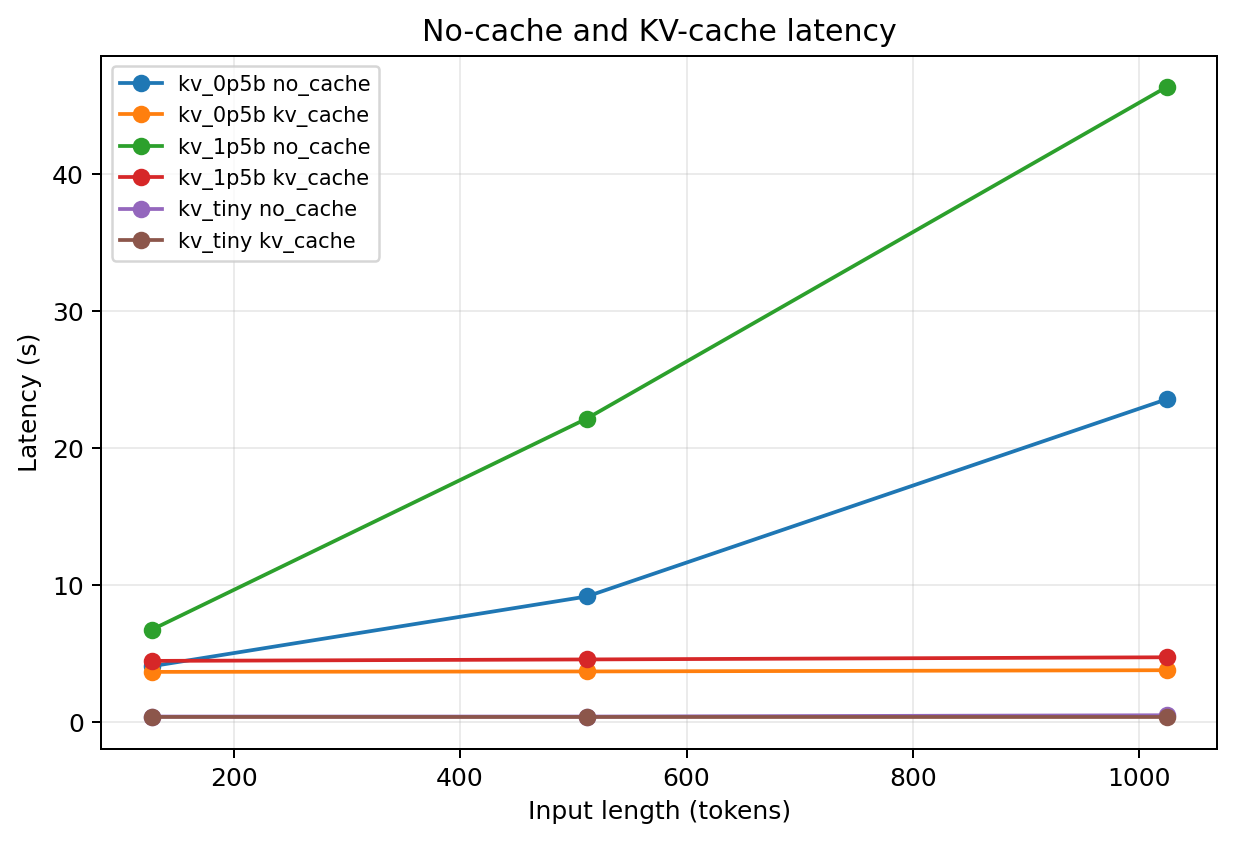
\includegraphics[width=\columnwidth]{kv_latency.png}
\caption{Full-prefix and KV-cache latency on synthetic token IDs.}
\label{fig:kv-latency}
\end{figure}
\begin{figure}[t]
\centering
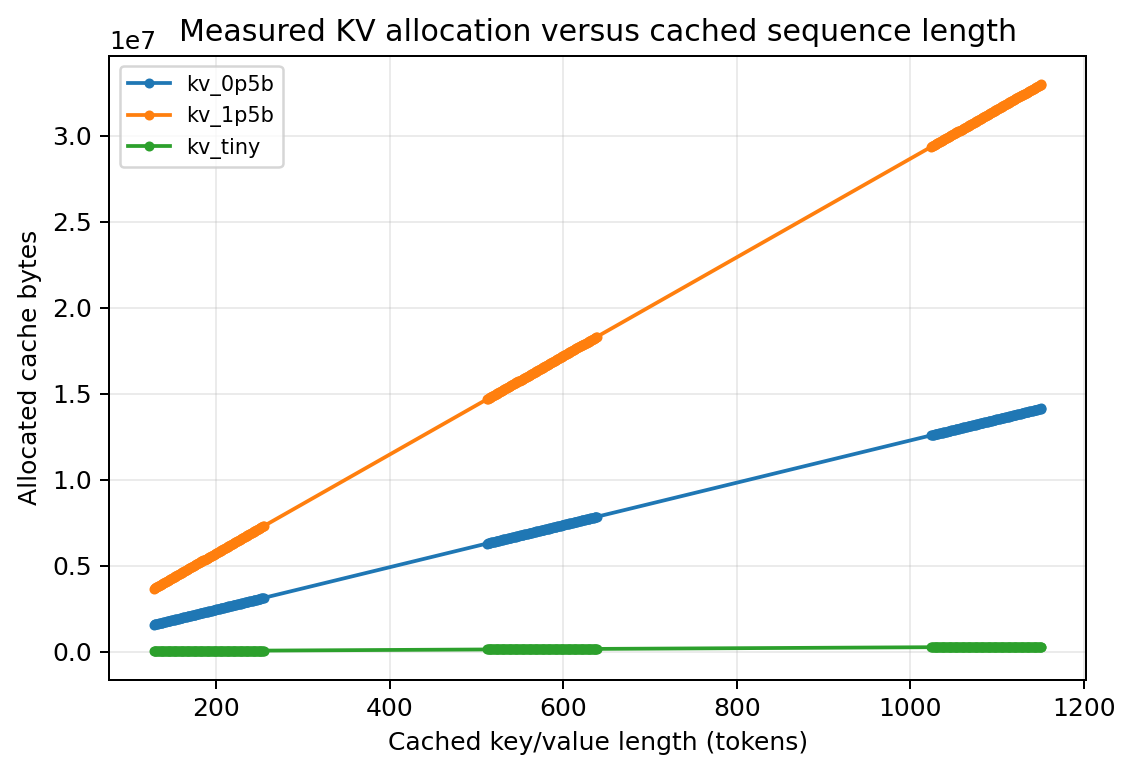
\includegraphics[width=\columnwidth]{kv_cache_growth.png}
\caption{Measured key/value allocation versus cached sequence length.}
\label{fig:kv-growth}
\end{figure}
\begin{figure}[t]
\centering
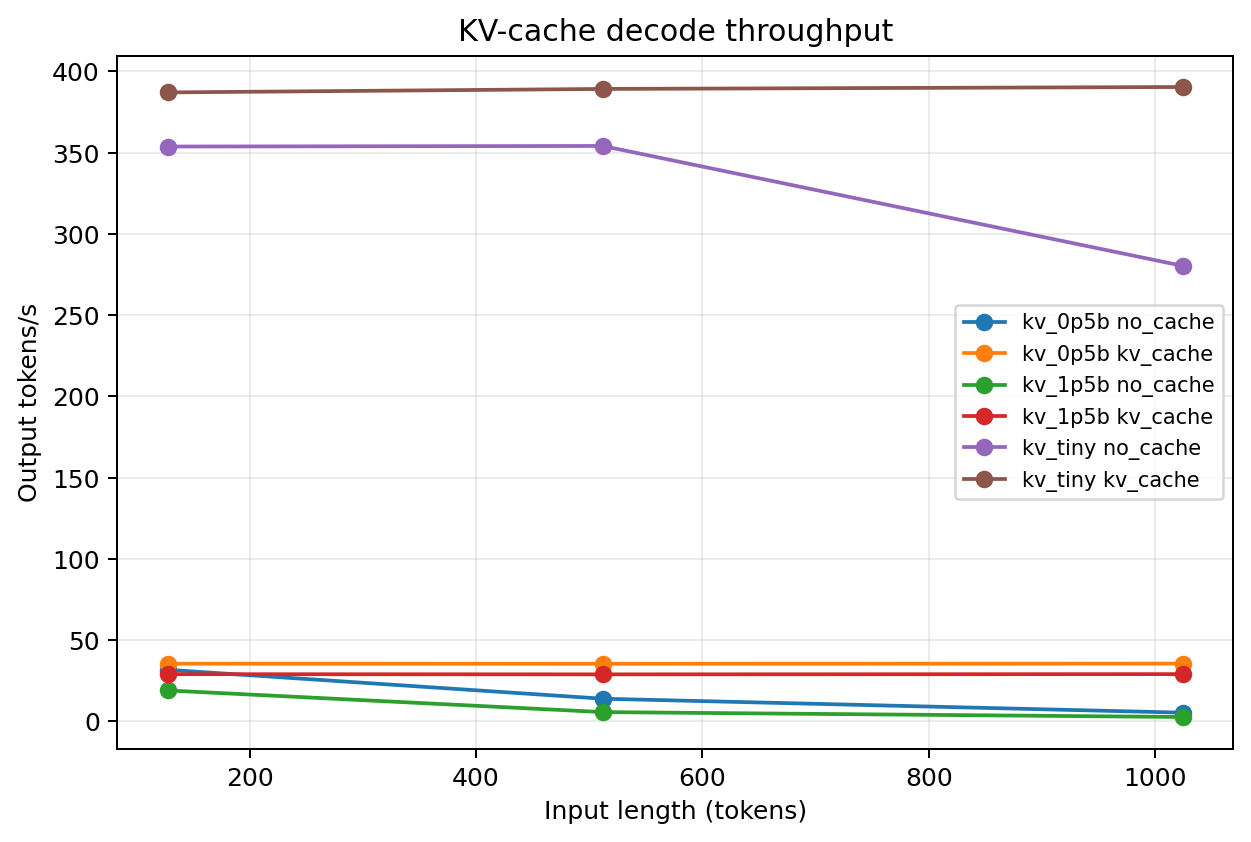
\includegraphics[width=\columnwidth]{kv_throughput.png}
\caption{KV-cache decode throughput on synthetic token IDs.}
\label{fig:kv-throughput}
\end{figure}
\begin{figure}[t]
\centering
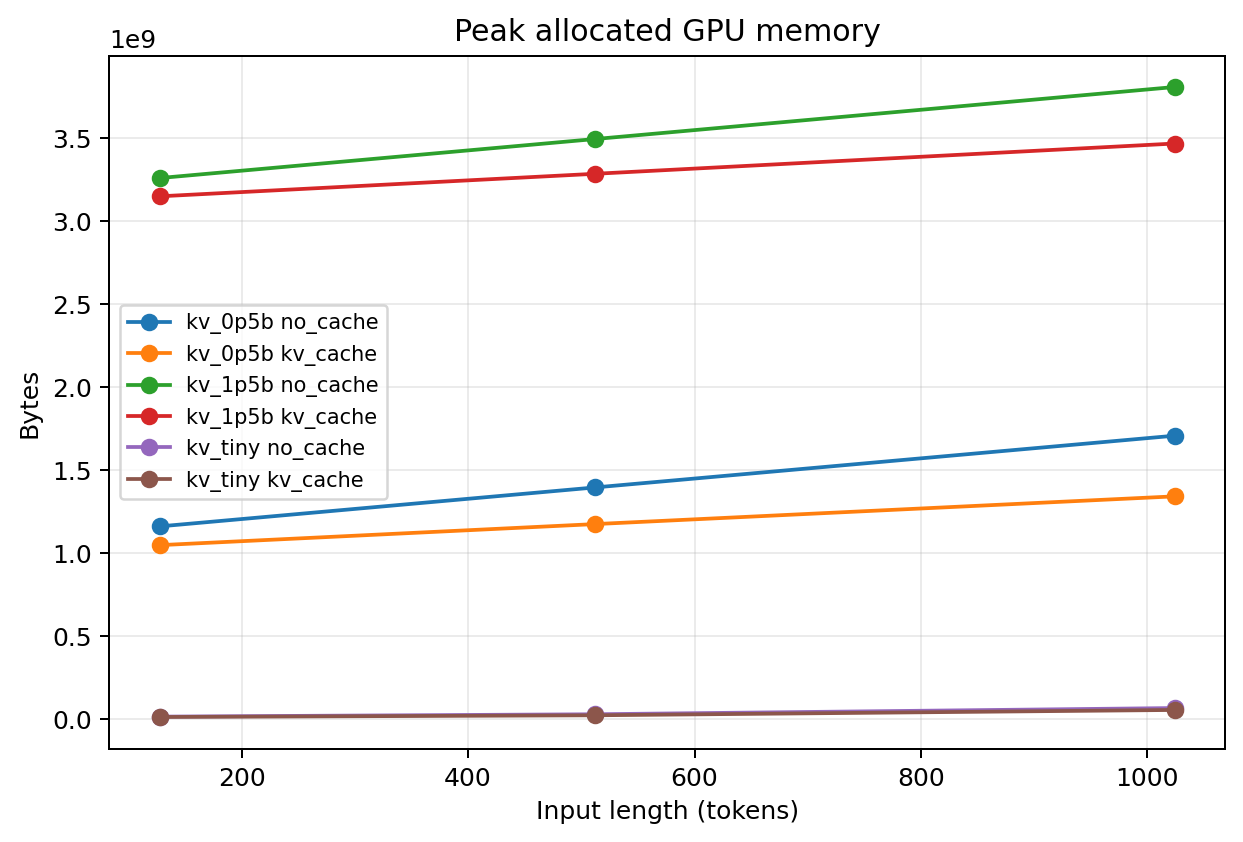
\includegraphics[width=\columnwidth]{kv_memory.png}
\caption{Peak memory allocation for no-cache and KV-cache decoding.}
\label{fig:kv-memory}
\end{figure}
\begin{figure}[t]
\centering
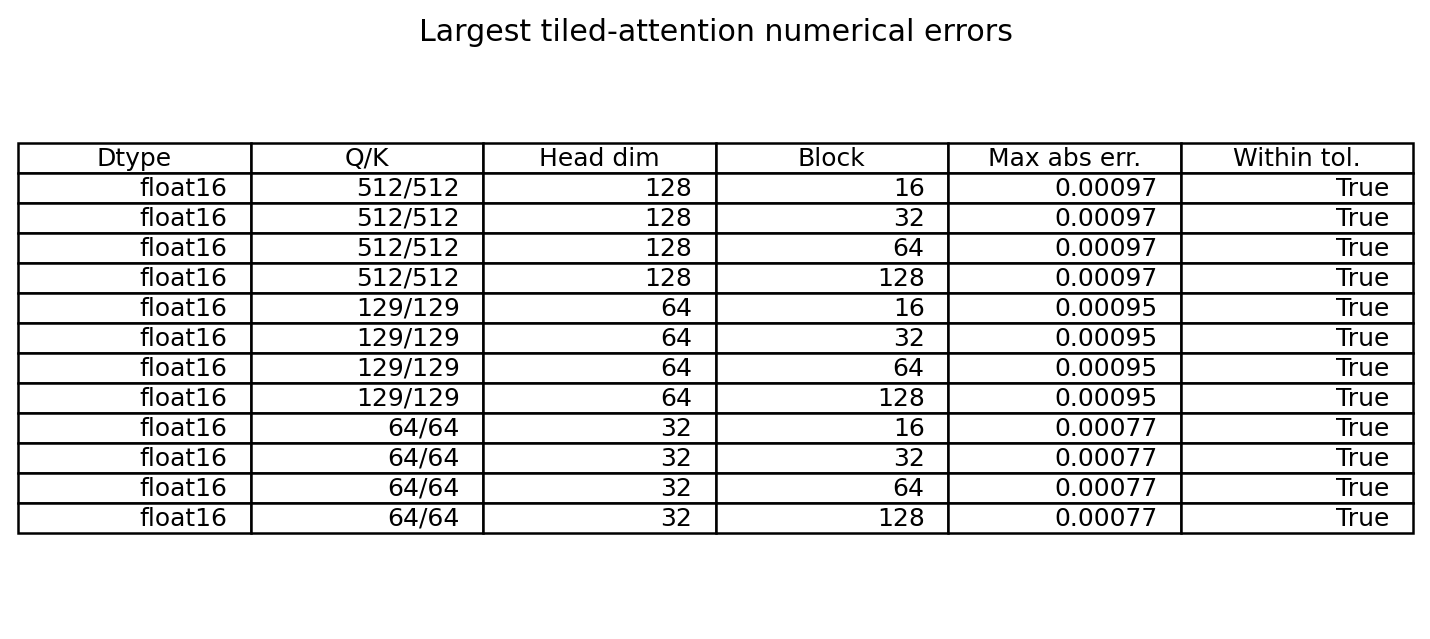
\includegraphics[width=\columnwidth]{attention_accuracy.png}
\caption{Worst observed numerical errors for tiled attention.}
\label{fig:attention-accuracy}
\end{figure}
\begin{figure}[t]
\centering
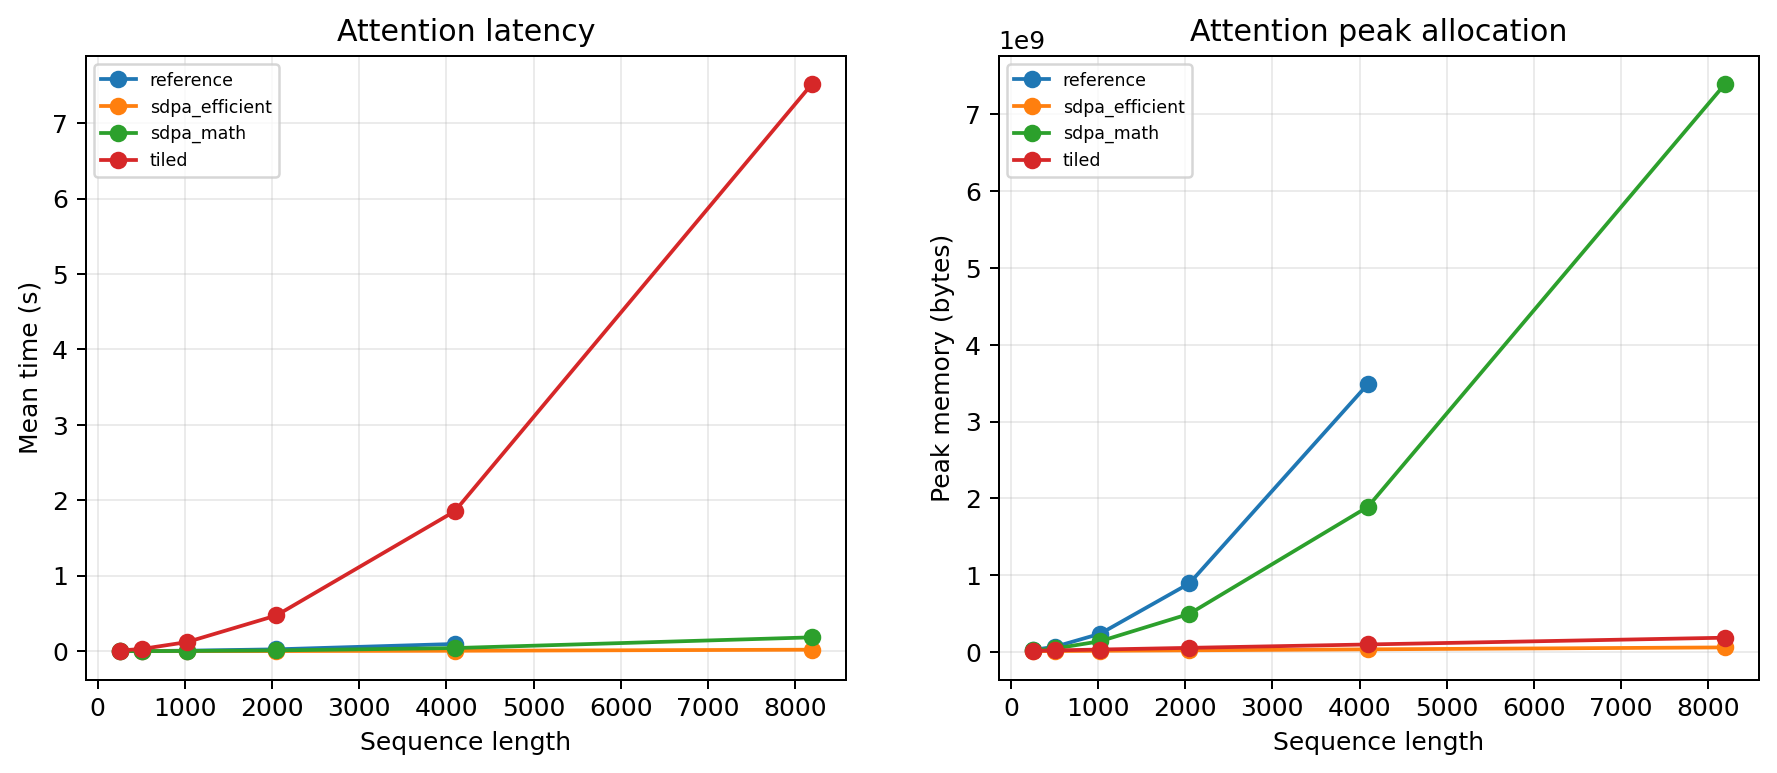
\includegraphics[width=\columnwidth]{attention_performance.png}
\caption{Tiled, reference, and available fused attention performance on synthetic tensors.}
\label{fig:attention}
\end{figure}
\begin{figure}[t]
\centering
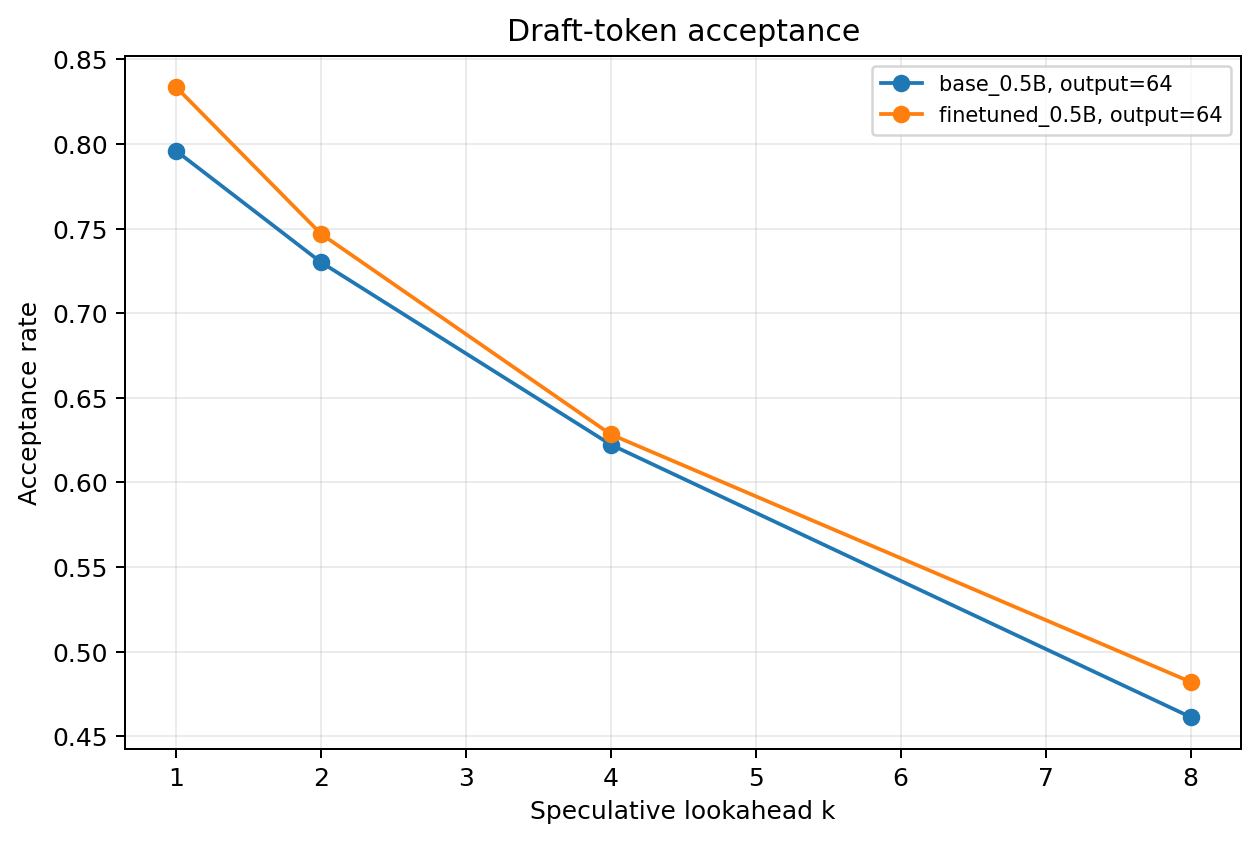
\includegraphics[width=\columnwidth]{speculative_acceptance.png}
\caption{Speculative draft-token acceptance by lookahead, draft model, and output length.}
\label{fig:spec-acceptance}
\end{figure}
\begin{figure}[t]
\centering
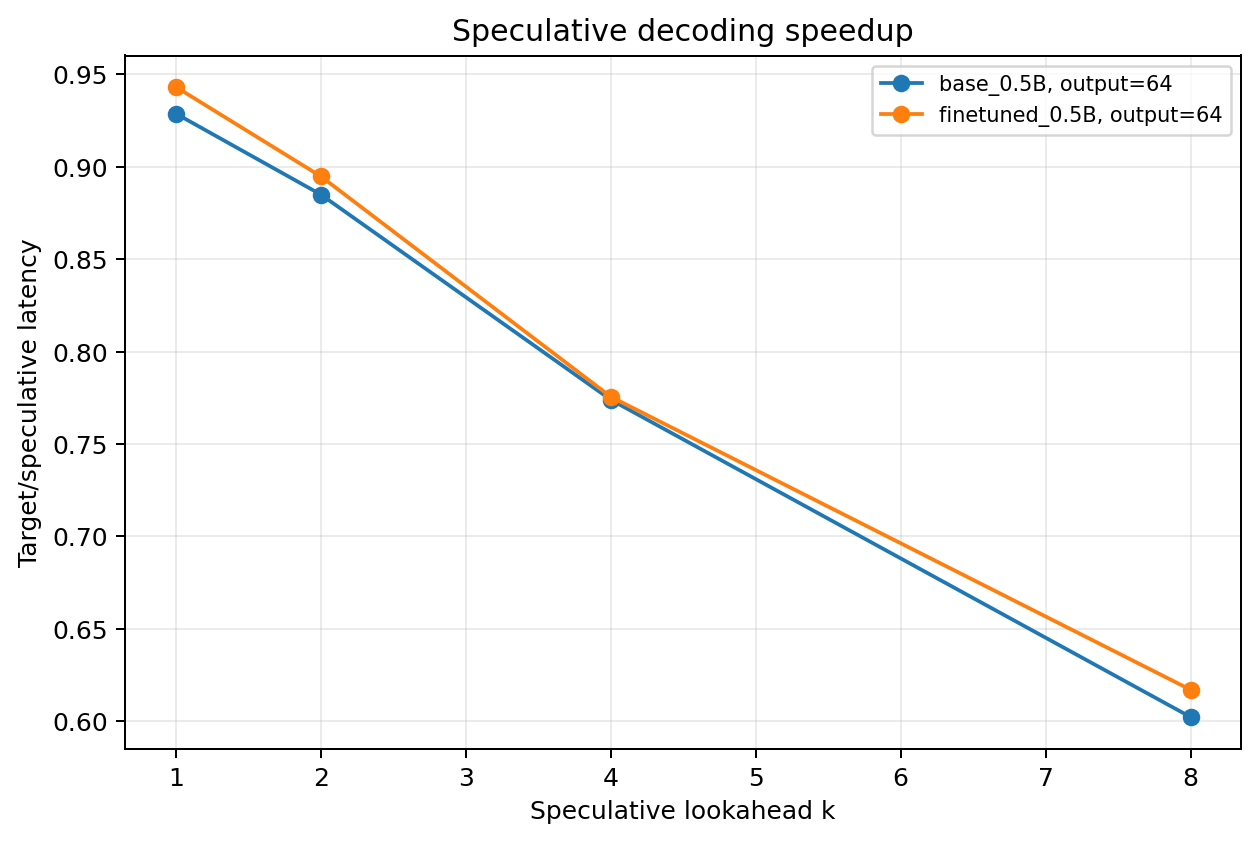
\includegraphics[width=\columnwidth]{speculative_speedup.png}
\caption{Measured target-to-speculative latency ratio; values below one indicate slowdown.}
\label{fig:spec-speedup}
\end{figure}
\begin{figure}[t]
\centering
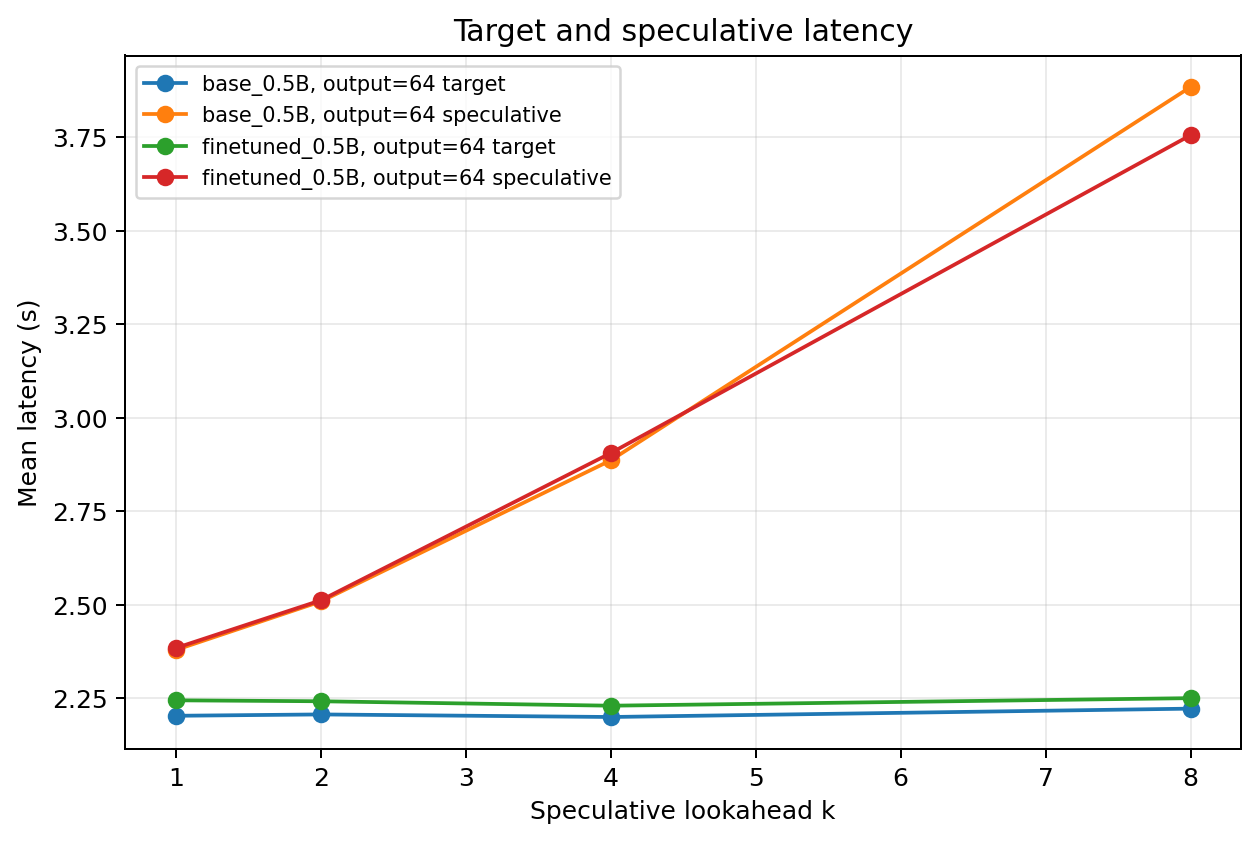
\includegraphics[width=\columnwidth]{speculative_latency_breakdown.png}
\caption{Target and speculative latency by lookahead.}
\label{fig:spec-latency}
\end{figure}

\subsection{Error analysis}
The automated error analyzer selects distinct candidate annotations from final predictions using label and evidence discrepancies. Its diagnoses are provisional, and note text is not copied into tracked report files. Table~\ref{tab:error-cases} summarizes candidates for author review; the full review worksheet is \texttt{docs/ERROR\_ANALYSIS.md}. The fine-tuned 1.5B model is wrong on 49 of 206 test criteria. Its errors are almost entirely \emph{abstention-boundary} errors; it never swaps the two decisive labels of a criterion (e.g., \emph{included} vs.\ \emph{not included}). The largest group (25 errors, 51\%) is \emph{not enough information} $\rightarrow$ \emph{not excluded} on exclusion criteria: the note does not mention a condition (e.g., a GFR threshold or previous axillary surgery), and the model treats absence as negation. This is the unsafe direction for screening, which is why decisive labels without cited evidence are routed to \emph{needs review}. The second group (7 errors) is \emph{not included} $\rightarrow$ \emph{not enough information}. For example, for ``patients undergoing elective carotid endarterectomy'' the model cites the correct procedure sentence but does not conclude that a different procedure fails the criterion; it never predicts \emph{not included} on the test set. Further cases involve qualitative versus numeric thresholds (``tachycardic'' for heart rate $\geq 90$), conditional criteria (``if female, using birth control''), and \emph{not applicable} versus \emph{not excluded} on sex-specific criteria, where expert labels themselves are inconsistent. In 27 correctly labelled rows the cited evidence differs from the expert set, so label accuracy overstates explanation quality.
\begin{table*}[t]
\centering
\scriptsize
\caption{Provisional error candidates for author review; note text is omitted.}
\label{tab:error-cases}
\begin{tabularx}{\textwidth}{rllX}
\toprule
ID & Variant/type & Gold $\rightarrow$ predicted & Candidate analysis \\
\midrule
169 & ft\_1p5b/exclusion & not enough information $\rightarrow$ not excluded & missing\_information\_guess, unsupported\_decision: The expert label is not-enough-information while the model made a decisive judgment; inspect whether the note actually supports that judgment. The output marks a decisive judgment without cited evidence; this should remain a manual-review case. \\
174 & ft\_1p5b/exclusion & not enough information $\rightarrow$ not excluded & missing\_information\_guess, unsupported\_decision: The expert label is not-enough-information while the model made a decisive judgment; inspect whether the note actually supports that judgment. The output marks a decisive judgment without cited evidence; this should remain a manual-review case. \\
179 & ft\_0p5b/exclusion & not excluded $\rightarrow$ not excluded & unsupported\_decision, missed\_gold\_evidence: The output marks a decisive judgment without cited evidence; this should remain a manual-review case. The cited evidence does not overlap the expert evidence; inspect the sentence numbering and whether the model missed the supporting fact. \\
166 & ft\_1p5b/exclusion & not excluded $\rightarrow$ not excluded & evidence\_set\_discrepancy: The model cited sentence IDs outside the expert evidence set; assess relevance locally because expert evidence may not be exhaustive. \\
193 & ft\_1p5b/exclusion & not enough information $\rightarrow$ not excluded & missing\_information\_guess, unsupported\_decision, missed\_gold\_evidence: The expert label is not-enough-information while the model made a decisive judgment; inspect whether the note actually supports that judgment. The output marks a decisive judgment without cited evidence; this should remain a manual-review case. The cited evidence does not overlap the expert evidence; inspect the sentence numbering and whether the model missed the supporting fact. \\
307 & ft\_1p5b/inclusion & not enough information $\rightarrow$ not enough information & evidence\_set\_discrepancy: The model cited sentence IDs outside the expert evidence set; assess relevance locally because expert evidence may not be exhaustive. \\
190 & ft\_0p5b/inclusion & not enough information $\rightarrow$ not enough information & evidence\_set\_discrepancy: The model cited sentence IDs outside the expert evidence set; assess relevance locally because expert evidence may not be exhaustive. \\
305 & ft\_1p5b/inclusion & not enough information $\rightarrow$ not enough information & evidence\_set\_discrepancy: The model cited sentence IDs outside the expert evidence set; assess relevance locally because expert evidence may not be exhaustive. \\
315 & base\_1p5b/exclusion & not enough information $\rightarrow$ excluded & missing\_information\_guess, evidence\_set\_discrepancy: The expert label is not-enough-information while the model made a decisive judgment; inspect whether the note actually supports that judgment. The model cited sentence IDs outside the expert evidence set; assess relevance locally because expert evidence may not be exhaustive. \\
323 & ft\_0p5b/inclusion & not enough information $\rightarrow$ included & missing\_information\_guess: The expert label is not-enough-information while the model made a decisive judgment; inspect whether the note actually supports that judgment. \\
325 & ft\_1p5b/inclusion & not enough information $\rightarrow$ not enough information & evidence\_set\_discrepancy: The model cited sentence IDs outside the expert evidence set; assess relevance locally because expert evidence may not be exhaustive. \\
389 & ft\_1p5b/exclusion & not enough information $\rightarrow$ not excluded & missing\_information\_guess, unsupported\_decision: The expert label is not-enough-information while the model made a decisive judgment; inspect whether the note actually supports that judgment. The output marks a decisive judgment without cited evidence; this should remain a manual-review case. \\
\bottomrule
\end{tabularx}
\end{table*}


\section{Application, Deployment, and Limitations}
The Gradio application presents criterion screening, evidence, an inference lab, benchmarks, and offline results. It is officially deployed as a locally hosted browser application, which satisfies the assignment. On Windows, \texttt{run\_app.bat} starts the app; the first run downloads the selected public model. An optional temporary Gradio share link is intended only for defense-day remote access. The Hugging Face Space remains staged but was not deployed because the platform requires a PRO account for the selected 2026 hardware.

The dataset contains a limited number of patients and the held-out split is correspondingly small; bootstrap intervals are included to communicate uncertainty. Labels and evidence inherit the source annotation's limitations, while evidence disagreement may reflect incomplete annotation rather than a model error. Synthetic-token inference benchmarks do not predict clinical workload latency. The application uses deterministic templates rather than independently verified rationales, and its aggregation rule is explicitly preliminary. CriterionLens is not a clinical decision system, must not be used for enrollment decisions, and requires expert review of every case.

\section{Conclusion}
CriterionLens demonstrates a reproducible, evidence-oriented pipeline for criterion-level trial screening with small instruction models, together with explicit inference implementations and a locally hosted demonstration. The results are limited to a single public annotation source and a small patient-disjoint evaluation. The KV cache gave large measured gains that grow with context, whereas exact speculative decoding did not pay off with a 0.5B draft on a T4, which shows why inference optimizations must be measured on the target hardware. Further work should test additional cohorts, improve annotation review, and optimize inference with measured rather than assumed benefits. Any clinical use would require substantially broader validation, governance, and oversight.


\bibliographystyle{IEEEtran}
\bibliography{references}

\appendices
\section{Reproducibility}
The repository records the dataset revision, patient split manifest, training configurations, model identifiers, benchmark configurations, evaluation metrics, and the final-test access log. Fast tests run with \texttt{.venv\textbackslash Scripts\textbackslash python.exe -m pytest -q}. Result tables and figures are regenerated with \texttt{.venv\textbackslash Scripts\textbackslash python.exe scripts\textbackslash make\_figures.py --require-test --require-bench}. Training archives and model weights are excluded from Git; published adapters and merged models are linked from the project README.

\noindent\textbf{Artifacts.} Code and execution instructions: \url{https://github.com/SyedAshherMajid/criterion-lens} (Windows start-up: \texttt{run\_app.bat}). LoRA adapter (headline): \url{https://huggingface.co/Ashher123/criterion-lens-qwen2.5-1.5b-lora}; merged models: \url{https://huggingface.co/Ashher123/criterion-lens-qwen2.5-1.5b-merged} and \url{https://huggingface.co/Ashher123/criterion-lens-qwen2.5-0.5b-merged}. Split manifest: \texttt{data/splits/split\_manifest.json}. Benchmark logs: \texttt{results/bench/}. Demonstration video: \url{https://youtu.be/Z3mVr0ccfKE}.

\section{AI-use statement}
Claude assisted with requirements analysis and preparation of the design and execution plan. An AI coding assistant using Copilot SDK in VS Code assisted with implementation, tests, and documentation. Claude Code assisted in the final phase with running the frozen test evaluation and benchmarks on Kaggle, the error-analysis write-up, the results text of this paper, and the scripted, captioned screen recording of the demonstration. Experimental values in this paper are generated from the repository's recorded result files; citations are taken from the verified literature notes. The author remains responsible for reviewing the paper, the analysis, and every claim before submission.

\end{document}
